\documentclass[letterpaper,twocolumn,10pt, anonymous]{article}
\usepackage{usenix2019_v3}

\usepackage{amsmath}
\usepackage{filecontents}
\usepackage{tikz}
\usepackage{xspace}
\usepackage{listings}
\usepackage{xcolor}
\usepackage{textcomp}
\usepackage{graphicx}
\usepackage{caption}
\usepackage{subcaption}
\usepackage{todonotes}
\usepackage{multirow}
\usepackage{booktabs}
\usepackage{paralist}
\usepackage{enumitem}
\usepackage{tabulary}
\usepackage{prettyref}
\usepackage{verbatim}
\usepackage{balance}
\usepackage{tabularx}

%-------------------------------------------------------------------------------
\begin{document}
%-------------------------------------------------------------------------------


\lstdefinestyle{cstyle}{
  basicstyle=\footnotesize\ttfamily,
  keywordstyle=\color{black!85}\bfseries,
  keywordstyle=[2]\color{black!85}\bfseries\emph,
  showstringspaces=false,
  language={C},
  breaklines=false,
  mathescape=true,
  escapechar={@}
}
\lstdefinestyle{inline}{
  style=cstyle,
  mathescape=false,
  breaklines=true,
  keywordstyle=,           
  keywordstyle=[2],
  extendedchars=true,
  basicstyle=\ttfamily\small
}
\newcommand{\Code}[1]{\lstinline[style=inline,breaklines=false]@#1@}
\let\realparagraph\paragraph
\let\paragraph\relax
\newcommand{\paragraph}[1]{\textbf{#1.}}
\newcolumntype{Q}{>{\centering\arraybackslash}X}

\newcommand\tocttou[0]{ToCtToU\xspace}
\newcommand\tiktok[0]{TikTok\xspace}

\newrefformat{cha}{\hyperref[#1]{Chapter~\ref*{#1}}}
\newrefformat{sec}{\hyperref[#1]{Section~\ref*{#1}}}
\newrefformat{sub}{\hyperref[#1]{Section~\ref*{#1}}}
\newrefformat{tab}{\hyperref[#1]{Table~\ref*{#1}}}
\newrefformat{fig}{\hyperref[#1]{Figure~\ref*{#1}}}
\newrefformat{line}{\hyperref[#1]{line~\ref*{#1}}}
\newrefformat{lst}{\hyperref[#1]{Listing~\ref*{#1}}}
\newrefformat{pat}{\hyperref[#1]{Patch~\ref*{#1}}}
\newrefformat{alg}{\hyperref[#1]{Algorithm~\ref*{#1}}}

\newcommand\mat[1]{\noindent{\color{blue} {\bf \fbox{Mat}} {\it#1}}}
\newcommand\atri[1]{\noindent{\color{red} {\bf \fbox{AB}} {\it#1}}}

%don't want date printed
\date{}

% make title bold and 14 pt font (Latex default is non-bold, 16 pt)
\title{\Large \bf Kernel TOCTTOU Protection}

%for single author (just remove % characters)
\author{
{\rm Anonymous}\\
Your Institution
% copy the following lines to add more authors
% \and
% {\rm Name}\\
%Name Institution
} % end author

\maketitle

%-------------------------------------------------------------------------------
\begin{abstract}
%-------------------------------------------------------------------------------
Your abstract text goes here. Just a few facts. Whet our appetites.
Not more than 200 words, if possible, and preferably closer to 150.
\end{abstract}

\begin{figure}[]
  \centering
  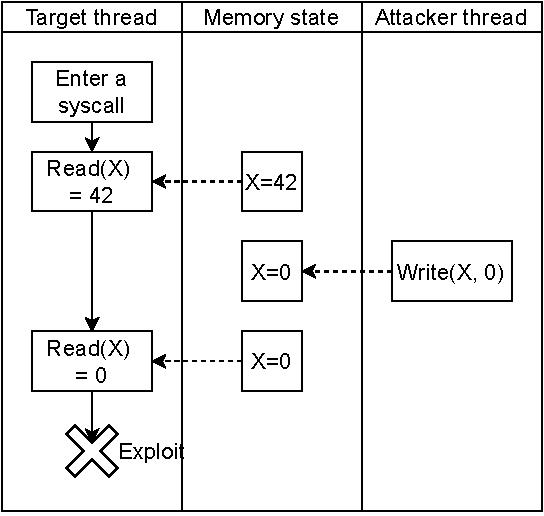
\includegraphics[width=.85\linewidth]{img/doublefetch.pdf}
  \caption{Example of a double-fetch bug}
  \label{fig:doublefetch}
\end{figure}

\section{Design}

\tiktok maintains a single core \emph{invariant}:
\textbf{\emph{Through a syscall's lifetime, every read to a userspace object 
will return the same value}}.
By construction, the invariant guarantees that double-fetches in syscall
code will read the same data, \emph{eliminating \tocttou bugs}.
\tiktok maintains the invariant by tracking \emph{snapshots} of objects
when first accessed, lazily making \emph{copies} when the object is concurrently 
written and accessing the correct copy on subsequent reads.
Copies are only maintained during syscalls' lifetimes, and are released as 
soon as no syscall needs it.
Consequently, each userspace object has a single copy when no syscalls are
running.
The invariant also means that only accesses to userspace objects by the kernel
need to be protected. 
Accesses to userspace objects from userspace and kernel objects by kernel 
code remains unaffected.

In addition, \tiktok must assure \emph{correctness}: there must exist an
execution on a non-\tiktok system where userspace \emph{never} modifies data 
between double-fetches by the kernel which is identical to the execution
of syscalls protected by \tiktok.

\tiktok's implementation builds on the protection mechanisms provided by 
existing virtual memory implementations.
On modern platforms, virtual memory protection is set up by the OS at
page-granularity by setting bits in pagetable entries.
These permission bits are checked by the hardware on memory access, 
efficiently enforcing that the permissions are respected, or raising 
a fault when they are not.
Therefore, \tiktok implements its invariant at a page-granularity, not object 
granularity: when a syscall reads from userspace, every page touched by that 
read is covered by the invariant, not merely the bytes read.
As a side-effect of this implementation, \tiktok cannot differentiate between
accesses to different parts of a page, and may incur performance overhead due
to false sharing within a page. 
Page-granularity protections are more conservative compared to byte-granularity
protection, therefore \tiktok maintains its invariant nonetheless.

For an object spanning multiple pages, \tiktok's design sequentially 
protects each page before reading from it.
The leading pages containing the object are protected before the
later pages, allowing an attacker to potentially modify the later 
pages before the syscall first reads them.
However, the attacker is prevented from modifying any of these earlier pages
after the syscall's first read, ensuring that double-fetches respect
the invariant.
\mat{Argue that this is a 'wavefront' style of mitigation.}
If the syscall code contains a \tocttou bug, the modification will
be visible to the first fetch itself (which is used for checking for 
validity of the data) and will lead to the data being rejected 
straightaway.
\tiktok's invariant therefore prevents exploitation of double-fetch
vulnerabilities even when the fetched objects span multiple pages.

A major requirement for \tiktok is to allow concurrent access to pages
by user/kernel code running in parallel with a syscall which reads from 
the same pages.
This requirement prevents deadlocks and improves performance vis-a-vis
a na\"ive design which blocks all other tasks writing to pages already 
read by a syscall until the syscall completes.
The na\"ive design can deadlock because it introduces dependencies between
tasks for forward progress, and we illustrate this in the following example
of a system with two tasks, A and B.
Task A issues a blocking system call which reads a user page and blocks. 
Task B writes to the same user page before issuing a syscall which 
resumes task A. 
In this case, if Task A's read to the page preceeds Task B's write, 
Task B will be blocked waiting for A to complete its syscall.
Task A will also remain blocked waiting for Task B's syscall, 
introducing a circular dependency, leading to deadlock.
The na\"ive design also introduces unnecessary delays in other cases, 
such as the one described below, again with two tasks C and D.
Task C reads from a page and sleeps for a long, determinate while.
Task C does not read from the page a second time.
Task D writes to the same page after task C has read from it, and 
blocks until Task C completes and is unnecessarily delayed.
A more performant approach is to duplicate the page: the copy is 
kept should task C fetch data from the page again, and task D
can write to the original and proceed without delays.
\atri{Maybe link to database optimistic concurrency control}

\tiktok must maintain multiple versions of a page read by a syscall 
to maintain its invariant in the face of concurrent writes.
\tiktok introduces \emph{snapshots} and \emph{copies} to keep track 
of page versions. 
Snapshots are logical views of the page's contents at a particular time,
while the actual contents are stored in one of many copies. 
Each snapshot maps to a copy, allowing the contents of the page at the 
time of creating the snapshot to be read. 
If multiple snapshots are taken without intervening writes to the page, 
these snapshots will map to a single copy, reducing \tiktok's space overheads 
and performance overheads for creating copies.
\tiktok maintains a snapshot of every page when first read by a syscall.
On a double fetch by the same syscall, the copy mapped to by the snapshot 
is accessed ensuring that the data read is the same as the first time.
The latest copy of the page is used for all writes, by the syscall as 
well as from concurrently running tasks, updating the page as seen 
from userspace.
Essentially, \tiktok is a multi-versioning system for pages where 
syscalls read from immutable versions to prevent \tocttou bugs and
syscalls and userspace both write to a single mutable version 
holding the latest state of the page.

\subsection{Page state machine}

\begin{figure*}[]
  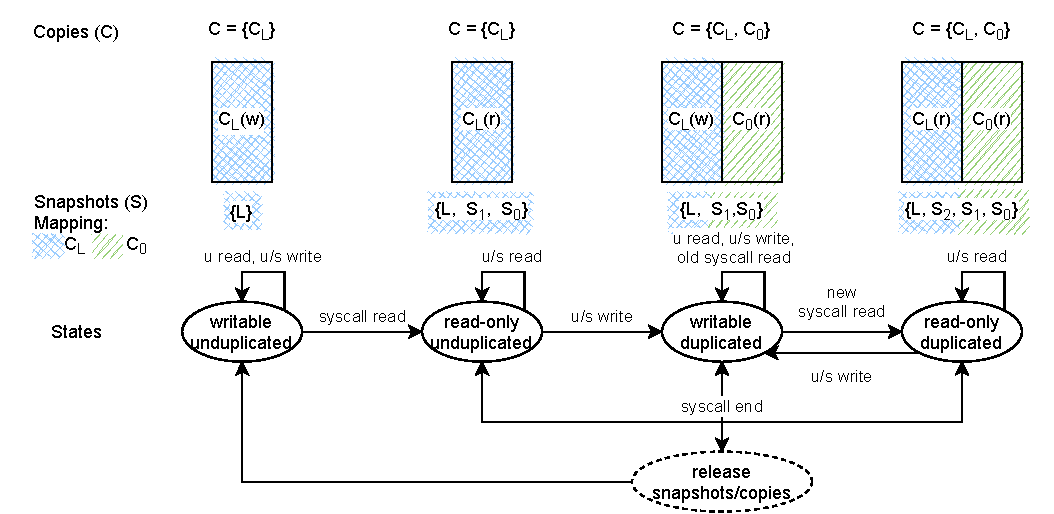
\includegraphics[width=\linewidth]{img/tiktok_states.pdf}
  \caption{State diagram for a page in \tiktok. Reads/writes from userspace/syscall 
          code are marked (u)/(s) respectively.}
  \label{fig:tiktok_states}
\end{figure*}

\begin{figure}[]
  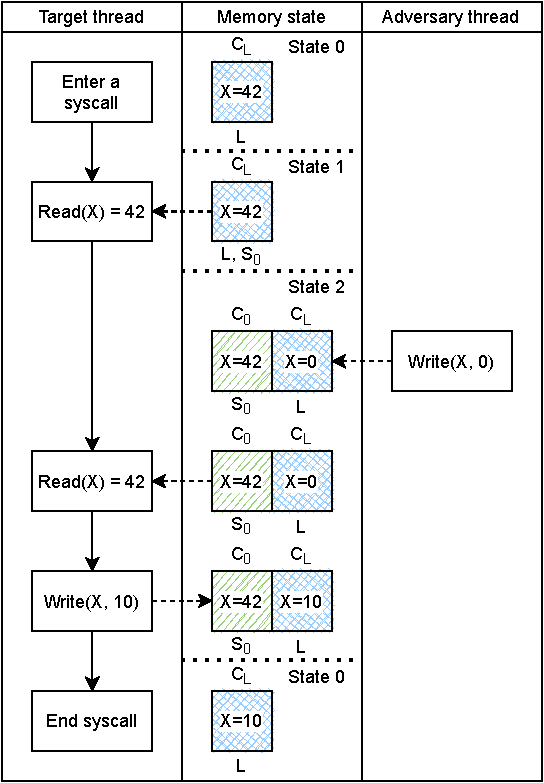
\includegraphics[width=\linewidth]{img/doublefetch_tiktok.pdf}
  \caption{Diagram illustrating \tiktok preventing exploitation of a double fetch.}
  \label{fig:doublefetch_tiktok}
\end{figure}

To track multiple versions of the contents of a page when being concurrently 
accessed by numerous tasks, from userspace or during a syscall,
\tiktok implicitly maintains a per-user-page state machine.
For each page, its corresponding state machine 
\begin{inparaenum}
  \item tracks snapshots for currently executing syscalls which have read it, 
  \item tracks copies of the page, and 
  \item maintains the mapping between snapshots and copies necessary for providing 
  the correct contents to subsequent reads by these syscalls.
\end{inparaenum}

\autoref{fig:tiktok_states} shows the state machine for a single page.
At every state, the page has two associated sets:
\begin{inparaenum}[\itshape i\upshape)]
  \item the copies set $C = \{C_L, C_0, \dots\}$ holds multiple copies of the page over time, and
  \item the snapshots set $S = \{L, S_0, S_1, \dots\}$ tracks logical versions of the page, each corresponding to one executing syscall and mapping to a copy. 
\end{inparaenum}
Reads from kernel code in a syscall use the copy corresponding to its snapshot.
Writes from user/kernel code and reads from userspace access the latest 
copy, which is mapped in process' address spaces.
\TODO{Should I formally define this mapping?}
All other copies are read-only (no matter what the original page protection is), and are used for providing snapshots to syscalls.
Read-only pages only use states 0 and 1, and writes lead to segmentation faults
as they do on non-\tiktok systems.
The latest copy $C_L$ of read-only pages remains read-only in both states.
In the following paragraphs, we describe how the state machine for a single, 
writable user page transitions between its states, what triggers each transition, 
and what changes are made to the copies and snapshot sets on a transition.
In \autoref{fig:doublefetch_tiktok}, we illustrate how the state machine protects the 
syscall from \autoref{fig:doublefetch}.

\paragraph{State 0}
A page starts as \texttt{(unprotected, unduplicated)}.
In this state, there is a single copy $C_L$ and a single ``snapshot'' $L$. 
The snapshot $L$ refers to the latest version of the page which changes 
with time, and is the only mutable snapshot.
All processes where this page is mapped have unrestricted userspace read and write 
access, and unrestricted kernel write access.
The remaining operation, a read from kernel code, triggers a transition to 
the next state.
In \autoref{fig:doublefetch_tiktok}, we see the snapshot $L$ initially containing 
the value $42$.

\paragraph{State 1}
The page in State 0 transitions to the \texttt{(protected, unduplicated)} state as soon as a syscall 
reads from it.
\tiktok first marks the page's latest copy $C_L$ read-only in all processes, 
trapping writes to the page but allowing concurrent userspace reads to continue.
A new snapshot, $S_0$ linked to this syscall is allocated for this page.
For the rest of its lifetime, this syscall will only read from this snapshot.
Both snaphots $S_0$ and $L$ refer to the same copy $C_L$ (shown by the 
blue cross-thatch in \autoref{fig:tiktok_states}).
Prior to any writes to this page, any other syscalls which also read the page  
get their own snapshots (e.g., $S_1$) all pointing to the single copy $C_L$.
The page's read-only status causes the hardware to fault on any write,
notifying \tiktok to transition the page to the next state.
In \autoref{fig:doublefetch_tiktok}, the page transistions to state 1 when 
the syscall first reads it, and adds a snapshot $S_0$.

\paragraph{State 2}
A page in State 1 transitions to (unprotected, duplicated) on any write from 
user or kernel code.
\tiktok duplicates the latest copy $C_L$, creating a new copy $C_0$ holding
the contents of the page prior to the write.
\tiktok moves all snapshots except $L$ (i.e. $S_0$ and $S_1$) previously 
pointing to $C_L$ to now point to the new copy $C_0$ (shown by green shading 
in \autoref{fig:tiktok_states}). 
Thereafter, the latest copy $C_L$ is made writable, and the triggering write 
is retried. 
Note how, at this state, any read using the snapshots $S_0$ or $S_1$ reads 
from the unmodified copy $C_0$ while writes directly affect $C_L$.
Certain syscalls such as \Code{rt_sigaction} both read and write from 
the same user page. 
A write by \Code{rt_sigaction} to the page it has previously read will update
the page's latest copy $C_L$, but not the duplicate copy $C_0$.
This ensures that the copy $C_L$ always holds the latest contents of the page, 
up-to-date with all the writes to the page, from both user and kernel code. 
Further, \tiktok does not need to merge writes from userspace and syscall code
on a syscall's completion, since both directly modify the same copy $C_L$.
All other copies $C_i$ are immutable.
When the attacker writes to the page in \autoref{fig:doublefetch_tiktok}, the
page moves to state 2, linking the snapshot $S_0$ to a copy holding the 
original value $42$.
The writes from both the adversary and the syscall itself both affect 
the copy $C_L$, but the read from the syscall accesses the snapshot $S_0$
and reads the same value as the first time.


\paragraph{State 3}
A separate syscall subsequently reading the page in State 2 transitions 
it to \texttt{(protected, duplicated)} state. 
The new snapshot, $S_2$, points to the latest copy $C_L$.
On a write, the page will be duplicated and this snapshot 
will point to the new copy (similar to that in state 2).

\paragraph{Releasing snapshots}
\tiktok uses snapshots to enable a syscall to read the same data from a page 
during its lifetime and releases snapshots when syscalls complete. 
Releasing a snapshot is possibly accompanied by a state transition
and the release of the mapped copy.
If $S_i$ mapped to the latest copy $C_L$, \tiktok cannot free the copy
since userspace is using it.
In this case, the page must be in state 1 or 3, and $C_L$ is read-only.
After removing $S_i$, if $L$ is the sole remaining snapshot mapped to $C_L$, 
\tiktok makes the page writable, moving to states 0 or 2 from states 
1 or 3 respectively. 
If $S_i$ is mapped to any other duplicate $C_i$, \tiktok frees the copy along
with the snapshot if $S_i$ is the last remaining snapshot mapped to $C_i$.
If the page was in state 2, $C_L$ was writable and unmapped by any snapshot,
so \tiktok changes the page to state 0.
This transitions is shown in \autoref{fig:doublefetch_tiktok}, where the 
snapshot $S_0$ and the copy $C_0$ are both discarded.
If the page was in state 3, $C_L$ was read-only and mapped by some other
snapshot, so \tiktok moves the page to state 1.

Under \tiktok, all writes are affected on to a single copy of the page $C_L$,
maintaining correctness for syscalls writing concurrently to the page while
eliminating the need for merging snapshots when syscalls complete.
On non-\tiktok systems, writes to a page from syscalls running concurrently
are interleaved onto the page based on what order these writes were 
executed. 
The same syscalls protected by \tiktok write to the latest snapshot $L$ (i.e. 
the copy $C_L$), and the final state corresponds to an interleaving of these
writes, just as in the non-\tiktok case.
The snapshots $S_i$ is immutable, can be dropped without requiring page 
merging, as described in the previous paragraph.


\subsection{Discussion}

\begin{table}
\begin{center}
\begin{tabularx}{\columnwidth} { | l | X |}
\hline
System Call & Exemption reason \\
\hline
\hline
\Code{futex} & Relies on concurrent write \\ \cline{1-2}
\Code{poll} & Relies on concurrent write \\ \cline{1-2}
\Code{ppoll} & Relies on concurrent write \\ \cline{1-2}
\Code{select} & Relies on concurrent write \\ \cline{1-2}
\Code{pselect6} & Relies on concurrent write \\ \cline{1-2}
\Code{rt\_sigtimedwait} & Relies on concurrent write \\ \cline{1-2}
\Code{execve} & Remaps address space \\ \cline{1-2}
\end{tabularx}
\end{center}
\caption{System calls uninstrumented by \tiktok}
\label{tab:except_syscall}
\end{table}
\paragraph{Exceptions}
Certain syscalls such as \Code{futex} rely on user data changing between 
double fetches to implement their functionality and cannot be protected by
\tiktok.
Such syscalls are listed in \autoref{tab:except_syscall}.
The \Code{futex} syscall implements a fast synchronization mechanism
for userspace and relies on atomic writes from concurrent userspace
threads to update a condition the syscall is waiting for. 
Subjecting a \Code{futex} syscall to \tiktok's invariant will prevent
it from ever waking up the waiting task.
Such syscalls cannot be protected by \tiktok, and we implement an 
exception list to prevent transitions in the state machines of pages read 
by these syscalls.
The code for these syscalls must be manually inspected for double-fetch 
vulnerabilities.
Crucially, exempting these syscalls from \tiktok's protection does not 
affect the security of other syscalls. 
Any writes from these syscalls are subject to the same rules described
in the state machine, and cannot break \tiktok's invariant.

Further, a hypothetical syscall which reads from an object, writes to it, and
then reads back the updated object cannot be protected using \tiktok.
\tiktok's invariant will ensure that the second read is identical to the first,
and does not reflect the intermediate write. 
The authors did not find any syscall which exhibits this behavior in the Linux
kernel. 
Such syscalls will also need to be exempted from \tiktok's instrumentation.

\paragraph{Preventing deadlocks in design}
\tiktok's design is free of deadlocks, and exempts syscalls which 
require violation of its invariant from triggering particular 
state-machine transitions.
Userspace reads always succeed, using the latest copy $C_L$ of the
accessed page.
Writes from userspace and kernel code succeed directly if the 
page is in states 0 or 2, and trigger a fault otherwise.
Handling these faults involves creating a new copy of the page and
setting the page writable. 
Reading from kernel code involves creating a new snapshot and 
setting the page read-only.
None of the aforementioned operations relies on other operations 
on the same page to complete and all are finite-time.
None of the operations on a page rely on operations on other pages.
A single, per-page lock can serialize operations on that page
and assure forward progress.


\todo{Discuss how Midgard would help}
\tiktok assumes that syscalls do not both read and write to the same user data. 
There are particular syscalls, however, which rely on such behaviour, and 
are not instrumented.

\todo{In implementation, discuss how IOMMU's can be used to prevent devide writes,
but is currently unsupported.}

Fake citation for compilation~\cite{silberschatz2018operating}.

\bibliographystyle{plain}
\bibliography{TikTok}

%%%%%%%%%%%%%%%%%%%%%%%%%%%%%%%%%%%%%%%%%%%%%%%%%%%%%%%%%%%%%%%%%%%%%%%%%%%%%%%%
\end{document}
%%%%%%%%%%%%%%%%%%%%%%%%%%%%%%%%%%%%%%%%%%%%%%%%%%%%%%%%%%%%%%%%%%%%%%%%%%%%%%%%

%%  LocalWords:  endnotes includegraphics fread ptr nobj noindent
%%  LocalWords:  pdflatex acks
